% region Done
\documentclass[a4paper, titlepage, final, 10pt]{article}
\usepackage{graphicx}
\usepackage[czech]{babel}
\usepackage[utf8x]{inputenc}
\usepackage[T1]{fontenc}
\usepackage[a4paper, top=3cm, bottom=2cm, left=1.5cm, right=1.5cm, marginparwidth=1.75cm]{geometry}
\usepackage{booktabs}
\usepackage[colorlinks=true, allcolors=blue]{hyperref}
\usepackage{fancyhdr}
\pagestyle{fancy}

\def\authorA{Jakub Čábera}
\def\titleA{ISS Projekt 2017/2018}

\title{\titleA}
\author{\authorA}

\lhead{\authorA}
\rhead{xcaber00}
\chead{\titleA}

\begin{document}
\section{Úkol 1}
	Vzorkovací frekvenci signálu: \textbf{16000Hz} \\
	Délku ve vzorcích: \textbf{16000} \\
	Délka v sekundách: \textbf{1s}
\section{Úkol 2}
	Výpočet \textit{logaritmické spektrální hustoty výkonu PSD} dle: \( G[k] = 10 \log_{10} \frac{|X[k]|^2}{N} \) \\
	PSD se mi zdálo přehlednější než pouze modul FFT.
	Vypočet \textit{frekvenční osy} dle: \( f = (0:N/2-1)/N \times FS \) \\
	Korekce počtu vzorků dle: \( G = G(1:N/2); \)

	{\centering 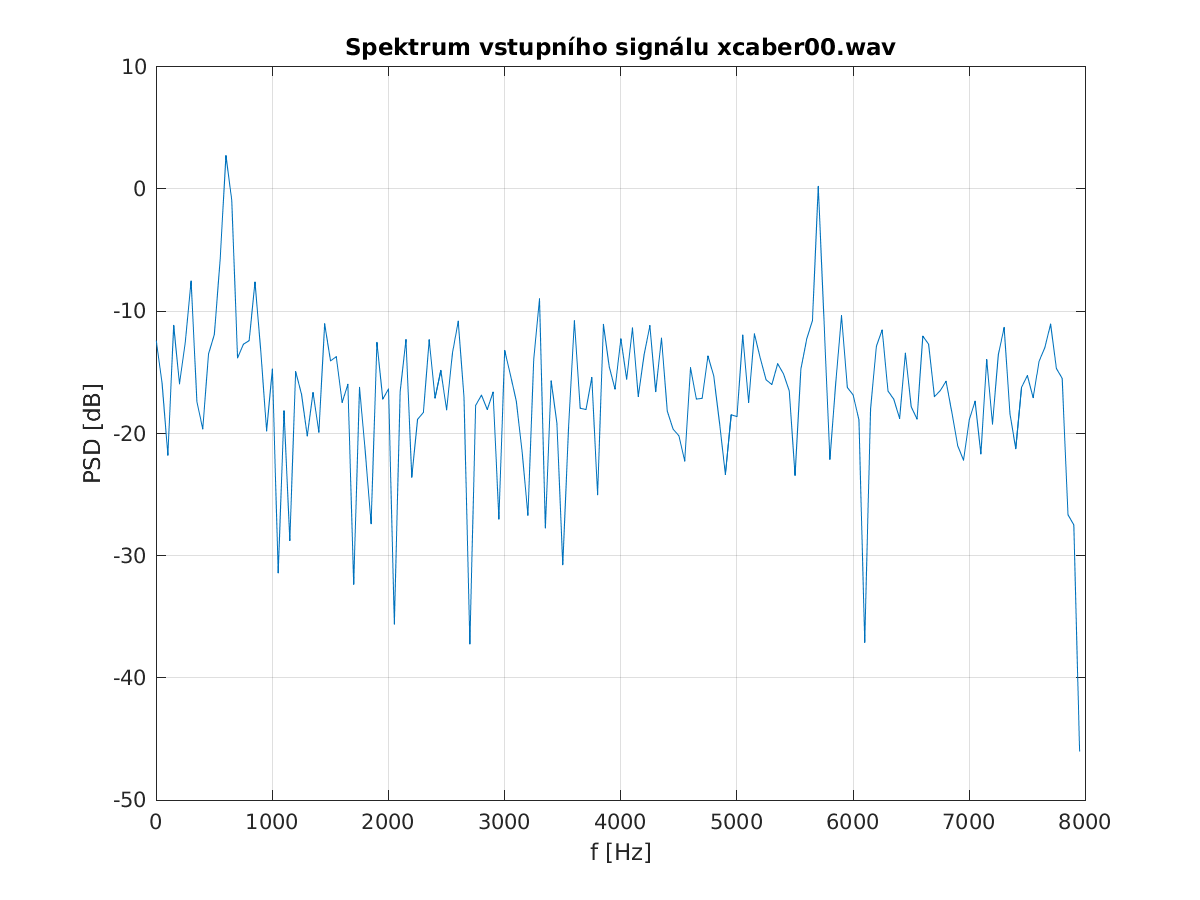
\includegraphics[width=\textwidth, height=7cm]{Final/task2.png} \par}
\section{Úkol 3}
	Maximum modulu spektra je na frekvenci \textbf{617 Hz}
\section{Úkol 4}
	Koeficienty filtru se vytisknout pomoc \textit{Zero-pole plot} funkce. \\
	Všechny Nuly a póly jsou uvnitř jednotkové kružnice => IIR Filtr je stabilní. (Při a0 = 1)

	{\centering 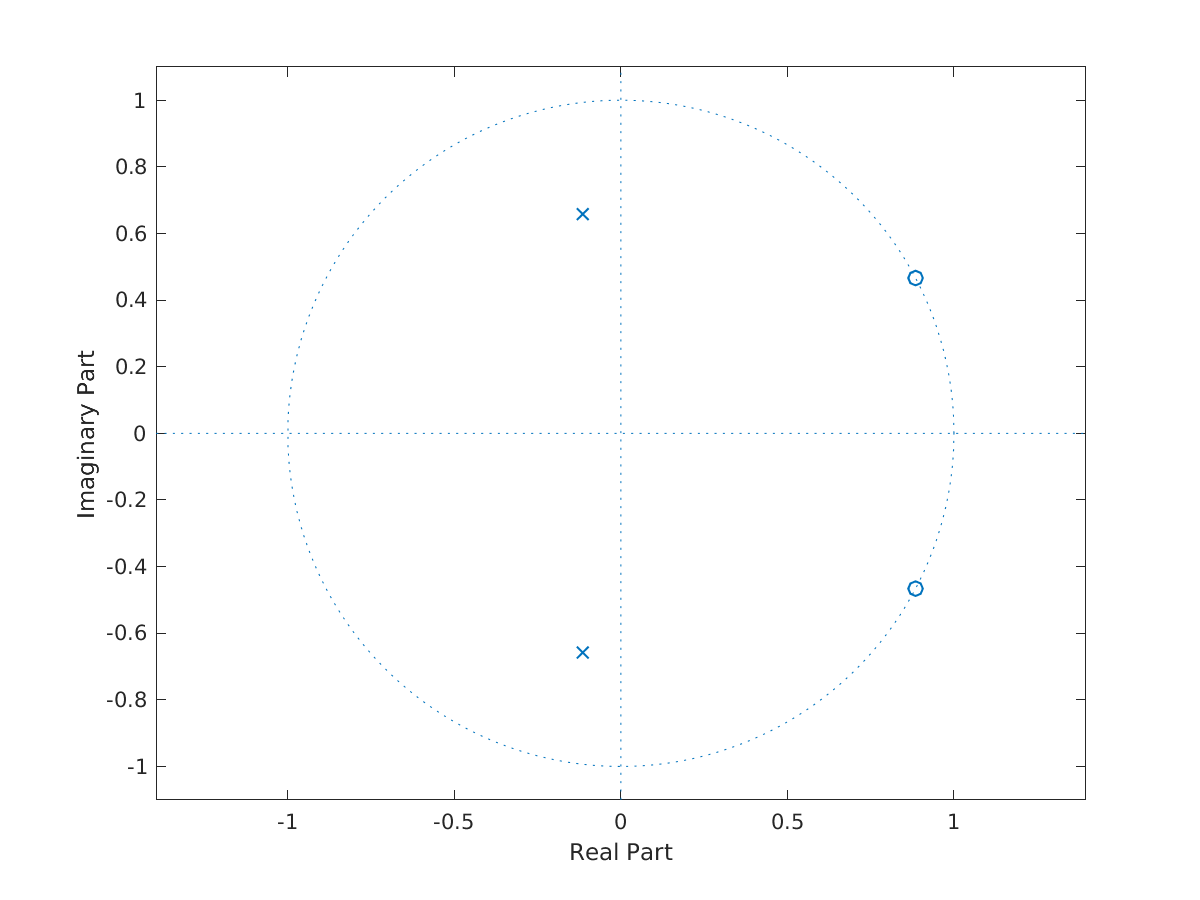
\includegraphics[width=\textwidth, height=8cm, keepaspectratio]{Final/task4.png} \par}
\section{Úkol 5}
	Jedná se o horní propust.

	{\centering 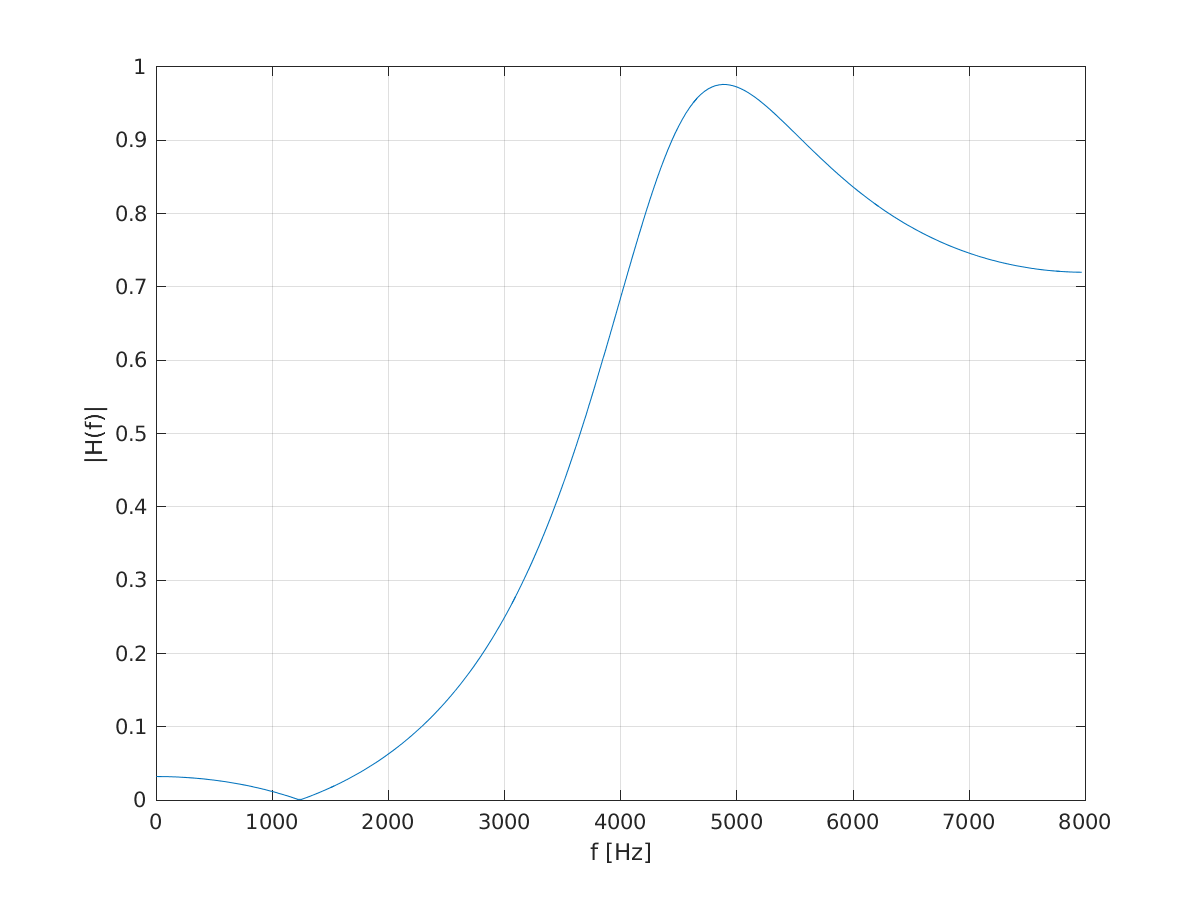
\includegraphics[height=8cm, keepaspectratio]{Final/task5.png} \par}
\section{Úkol 6}
	Zde jsem zvolil obyčejný linerání modul FFT.

	{\centering 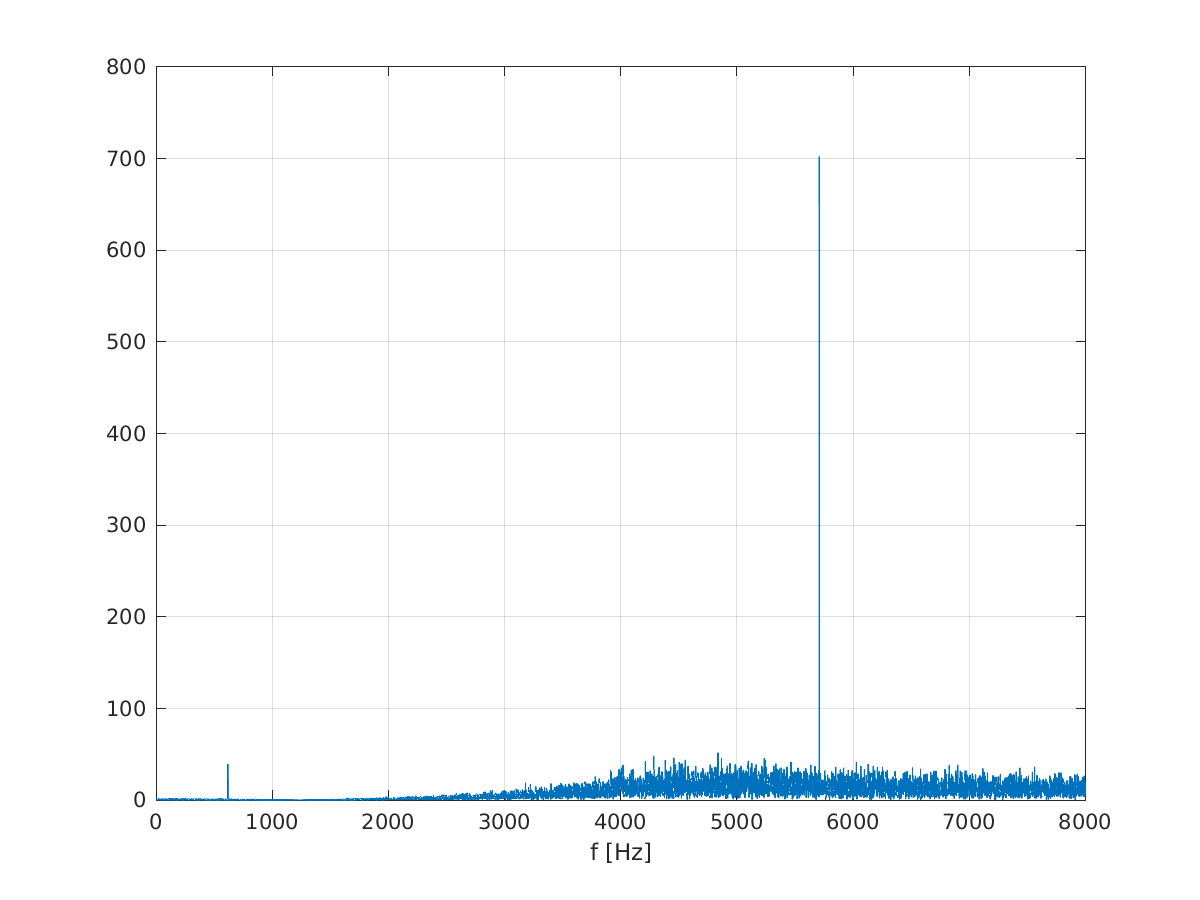
\includegraphics[width=\textwidth, height=7cm]{Final/task6.png} \par}
\section{Úkol 7}
	Maximum modulu spektra je na frekvenci \textbf{5709 Hz}
% endregion
\section{Úkol 8}
	Cosi
\section{Úkol 9}
	Nepovedlo se mi to pomocí funkce xcorr, tak jsem si funkci na odhad napsal sám dle:
	\( {R}(k) = \frac{1}{N} \sum_{n=0}^{N-1} x[n]x[n+k] \).

	{\centering 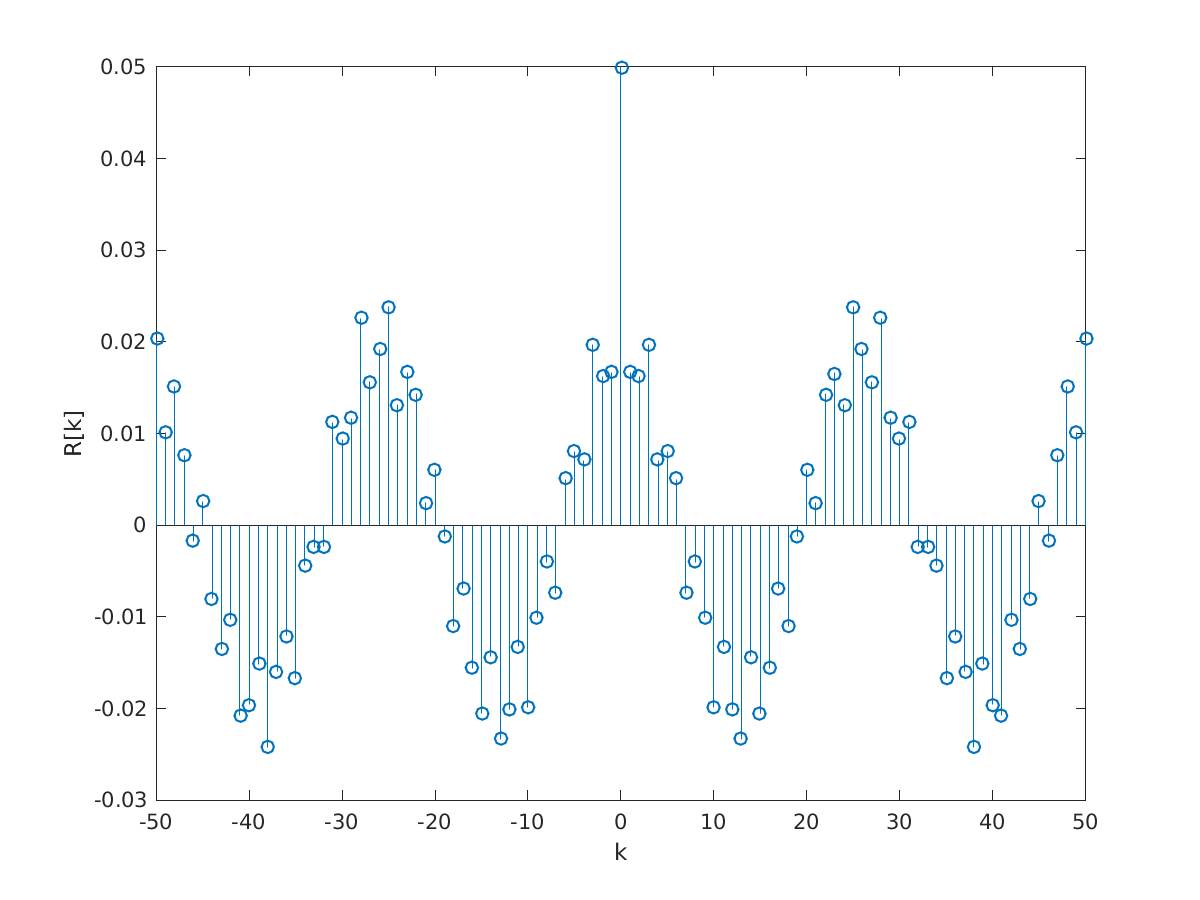
\includegraphics[width=\textwidth, height=7cm]{Final/task9.png} \par}
\section{Úkol 10}
	Hodnota R[10] je \textbf{-0.0207}.
\section{Úkol 11}
	Cosi
\section{Úkol 12}
	Jedná se o správnou sdruženou funkci hustoty rozdělení pravděpodobnosti.
\section{Úkol 13}
	Cosi

\end{document}
